\documentclass[12pt]{article}
\usepackage[left=2cm, right=2cm, top=2cm]{geometry}
\usepackage[utf8]{inputenc} 
\usepackage{mdframed} %For framing the title
\usepackage{graphicx} % to include images
\usepackage{amsmath} % For math mode
\usepackage{caption} % For captions
\usepackage{subcaption} % To use caption while using mini page
\usepackage{amssymb} % To use math symbols
\usepackage{multirow} %To combine multiple rows in a table
\usepackage[table]{xcolor} %To color rows / columns in table
\usepackage{titling} %To vertically center the title page
\usepackage{hyperref} %for URL


%----------------------------MATLAB TEMPLATE -------------------------------------
\usepackage{listings}
\usepackage{color} %red, green, blue, yellow, cyan, magenta, black, white
\definecolor{mygreen}{RGB}{28,172,0} % color values Red, Green, Blue
\definecolor{mylilas}{RGB}{170,55,241}
%-----------------------------------------------------------------------------------------

\title{ECE 8540 \\ Analysis of Tracking Systems \\ \quad \\
	Assignment 5 \\ Extended Kalman Filtering}
\author{Vivek Koodli Udupa \\ C12768888}
\date{October - 25, 2018 }

%%To make the title page center vertically centered
%\renewcommand\maketitlehooka{\null\mbox{}\vfill}
%\renewcommand\maketitlehookd{\vfill\null}

\begin{document}
\begin{mdframed}
%Displaying Title
%\begin{titlepage}
\maketitle
%\pagenumbering{gobble}% Remove page numbers (and reset to 1)
%\end{titlepage}
\end{mdframed}
\pagenumbering{arabic}% Arabic page numbers (and reset to 1)


%Begin of Report
\section{Introduction}
This report considers the problem of Extended Kalamn Filtering. In filtering, there are two prominent equations that describe the model that was designed to address a problem. The two equations are observation equation and state transition equation. The observation equation describes the measurements that are obtained through the sensors and the state transition equation describes how the system is expected to change over time. The Kalman filter is used to predict the future states of the system. But Kalman filter works only with functions that are linear. To solve non-linear functions, Extended Kalman Filter is used. \\ 
\\ \indent
Extended Kalman Filtering uses Taylor series expansion to get a linear approximation of the non-linear function. Taylor series works by taking a point and performing multiple derivatives at that point. In case of Extended Kalman Filter, mean of the Gaussian is taken on the non-linear curve and numerous derivatives are performed to approximate it. Only the first derivative of the Taylor series is considered while linearizing the non-linear curve. For every non-linear function, a tangent is drawn around the mean to try to approximate the function linearly. \\ 
\\ \indent
This report is focused on tracking something that is moving sinusoidally, like a spool of thread unwinding in a machine. Tracking the position of the spool from which the thread is originating would need a sinusoidal model because the thread position moves up and down as the spool unwinds, which is a sinusoidal motion when plotted over time. This report will include the methods and results of applying Extended Kalman filter to such a sinusoidal function.

\section{Methods}
Extended Kalman Filter(EKF) is a continuous cycle of predict and update. When formulating the problem for the EKF following steps are considered:
\begin{enumerate}
	\item Determine the state variables.
	\item Write the state transition equations i.e. How things evolve over time.
	\item Define the dynamic noise(s).  This describes the uncertainties in state transition equation.
	\item Determine the observation variables i.e. Sensor readings.
	\item Write the observation equations (relating the sensor readings to the state variables).
	\item Define the measurement noise(s). These are the uncertainties in observation variables.
	\item Characterize the state transition matrix and observation matrix.
	\item Check all matrices in the EKF equations to make sure the sizes are appropriate.
\end{enumerate}

\subsection{Deriving the equations for EKF sinusoidal model}
\label{sec: derivation}
It is difficult to formulate state transition equations for the sinusoidal problem mentioned in Introduction, because the dependent variable is expected to be time. For example: 
\begin{equation}
f(x_t,a_t) = \begin{bmatrix}
x_t = \sin \frac{t}{10} + a_t
\label{eq:sint}
\end{bmatrix}
\end{equation}
\indent
However, using equation \ref{eq:sint}, the following state does not depend upon the previous state; it only depends upon the time. This is not a viable formulation for state-space filtering, because there is no uncertainty in the state of the system with respect to time. \\
\\ \indent
However the state model and state transition equation can be modified to get something similar that can be used for filtering:
\begin{equation}
f(x_t,a_t) = \begin{bmatrix}
x_{t+1} = x_t + \dot{x}_t T \\
\dot{x}_{t+1} = \dot{x}_t + a_t \\
h_{t+1} = \sin \frac{x_t}{10}
\end{bmatrix}
\label{eq:sint mod}
\end{equation}
\indent
In equation \ref{eq:sint mod}. variable \textit{x} represents something like time and $\dot{x}$ along with dynamic noise $a_t$ represents uncertainty in the propagation of the sinusoid over time. The variable \textit{h} provides the actual value of the sinusoid. \\
\\ \indent
Using this model, three state variables are defined as:
\begin{equation}
X_t = \begin{bmatrix}
x_t \\
\dot{x}_t \\
h_t
\end{bmatrix}
\label{eq: xt}
\end{equation}
\indent
The state transition equations \ref{eq:sint mod} and \ref{eq: xt} given above, where $a_t$ is a random sample drawn from $N(0,\sigma_a^2)$ representing an uncertainty in the propagation of the sinusoid over time. \\
\\ \indent
For observation, the sensor that detects the current height of the sinusoid, $d_t$ will be considered:
\begin{equation}
Y_t = \begin{bmatrix}
d_t
\end{bmatrix}
\end{equation}
\indent
For example, this could be accomplished by using a light sensor to detect the thread position as it spins off a spool. The observation equations for this model are:
\begin{equation}
g(x_t,n_t) = \begin{bmatrix}
d_t = h_t + n_t
\end{bmatrix}
\end{equation}
\indent
where $n_t$ is a random sample drawn from $N(0,\sigma_n^2)$ representing measurement noise. \\
\\ \indent
In order to use this model in the EKF, four Jacobians must be calculated. The derivative of the state transition equations with respect to the state variables is: 
\begin{equation}
\frac{\partial f}{\partial x} =
\frac{\partial f}{\partial (x,\dot{x},h)} =
\begin{bmatrix}
1 & T & 0  \\
0 & 1 & 0  \\
\frac{1}{10} \cos \frac{x}{10} & 0 & 0 
\end{bmatrix}
\label{eq: Dfx}
\end{equation} \\
\\ \indent
The derivative of the observation equations with respect to the dynamic noises is:
\begin{equation}
\frac{\partial f}{\partial a} =
\frac{\partial f}{\partial (0,a_t,0)} =
\begin{bmatrix}
0 & 0 & 0  \\
0 & 1 & 0  \\
0 & 0 & 0 
\end{bmatrix} 
\label{eq: Dfa}
\end{equation}
\indent
The derivative of the observation equations with respect to the state variables is:
\begin{equation}
\frac{\partial g}{\partial x} =
\frac{\partial g}{\partial (x,\dot{x},h)} =
\begin{bmatrix}
0 & 0 & 1
\end{bmatrix}
\label{eq: Dgx}
\end{equation}
\indent
The derivative of the observation equations with respect to the measurement noises is:
\begin{equation}
\frac{\partial g}{\partial n} =
\frac{\partial g}{\partial (n_t)} =
\begin{bmatrix}
1 
\end{bmatrix}
\label{eq: Dgn}
\end{equation}
\\ \indent
The covariance of the dynamic noise is
\begin{equation}
Q = \begin{bmatrix}
0 & 0 & 0  \\
0 & \sigma_a^2 & 0  \\
0 & 0 & 0 
\end{bmatrix}
\label{eq: Q}
\end{equation}
\\ \indent
The covariance of the measurement noises is
\begin{equation}
R = \begin{bmatrix}
\sigma_n^2
\end{bmatrix}
\label{eq: R}
\end{equation}
\\ \indent
Equation \ref{eq:sint} through \ref{eq: R} theoretically describes the working of the EKF sinusoidal model. The implementation of the same will be described in the following section.

\subsection{Implementation}
As mentioned in section \ref{sec: derivation}  the EKF is a continuous predict and update loop and the equations for EKF has been derived. This section describes the implementation of above derived filter using the equations for the main loop.  \\
\begin{enumerate}
\item Predicting the next state: 
\begin{equation}
X_{t,t-1} = f(X_{t-1,t-1},0)
\label{eq:Xnext}
\end{equation}
where $f(X_{t-1,t-1},0)$ is the approximated state $\tilde{x}_t$. \\
\item Predicting next state covariance: 
\begin{equation}
S_{t,t-1} =
\left( \frac{\partial f}{\partial x} \right)
S_{t-1,t-1} \left(\frac{\partial f}{\partial x}\right)^T
+ \left( \frac{\partial f}{\partial a} \right) Q
\left(\frac{\partial f}{\partial a}\right)^T
\end{equation}
where $\left(\frac{\partial f}{\partial x}\right)$ and $\left(\frac{\partial f}{\partial a}\right)$ are the Jacobians of the state transition equations. \\
\\
\item Obtain measurement(s) $Y_t$ \\
\\
\item Calculate the Kalman gain (weights)
\begin{equation}
K_t = S_{t,t-1} 
\left( \frac{\partial g}{\partial x} \right)^T
\left[
\left( \frac{\partial g}{\partial x} \right)
S_{t,t-1}
\left( \frac{\partial g}{\partial x} \right)^T
+
\left( \frac{\partial g}{\partial n} \right)
R
\left( \frac{\partial g}{\partial n} \right)^T
\right]^{-1}
\end{equation}
where $\left(\frac{\partial g}{\partial x}\right)$ and $\left(\frac{\partial g}{\partial n}\right)$ are the Jacobians of the measurement equations.

\item Update state
\begin{equation}
X_{t,t} = X_{t,t-1} + K_t [Y_t - g(\tilde{x}_t,0)]
\end{equation}
where $g(\tilde{x}_t,0)$ is the ideal (noiseless) measurement of the approximated state from above.

\item update state covariance
\begin{equation}
S_{t,t} = \left[ I - K_t
\left( \frac{\partial g}{\partial x} \right) \right] S_{t,t-1}
\end{equation}

\item Now increment the loop iterator \textit{t}

\end{enumerate}
The implementation of the above described models and equations are done in MATLAB. Please refer appendix for the implementation code. 

\newpage
\section{Results}
This section consists of plots of EKF predictions against actual state and sensor measurement for various combinations of measurement noise(R) and dynamic noise(Q).  \\

The ratios of R and Q i.e measurement noise and dynamic noise decides what the filter output tend towards. One of the above mentioned noise is set to a certain value and the other is varied to see their effects. In this report, Q has been set to 0.001 and the R is varied. The plots for these combinations are given below. \\

Figure \ref{fig:EKF rat1} shows the output of the modeled EKF for high measurement noise of 1 and dynamic noise set to 0.001. Since the measurement noise is high, the filter output tends towards the true position and away from the measurement readings. \\

In Figure \ref{fig:EKF rat2} the measurement noise is decreased from 1 to 0.1. The filter output now balances between sensor measurement and true position. This seems to be the best combination of measurement noise and dynamic noise to fit the given data.\\

In Figure \ref{fig:EKF rat3} the measurement noise is further reduced to 0.03. Because of this reduction in measurement noise, the EKF filter now believes the sensor reading much more and this is evident in the EKF output, which is 
inclined towards the sensor reading. This can be seen clearly around sample 520 in Figure \ref{fig:EKF rat3} where the filter output is spiked in order to reach the sensor measurements. \\

%R = 1 Q = 0.001
\begin{figure}[b!]
\centering
	\includegraphics[width = \textwidth]{./Figures/ratio1.eps}
	\caption{EKF prediction for R = 1 and Q = 0.001}
	\label{fig:EKF rat1}
\end{figure}

%R = 0.1 Q = 0.001
\begin{figure}[ht!]
\centering
	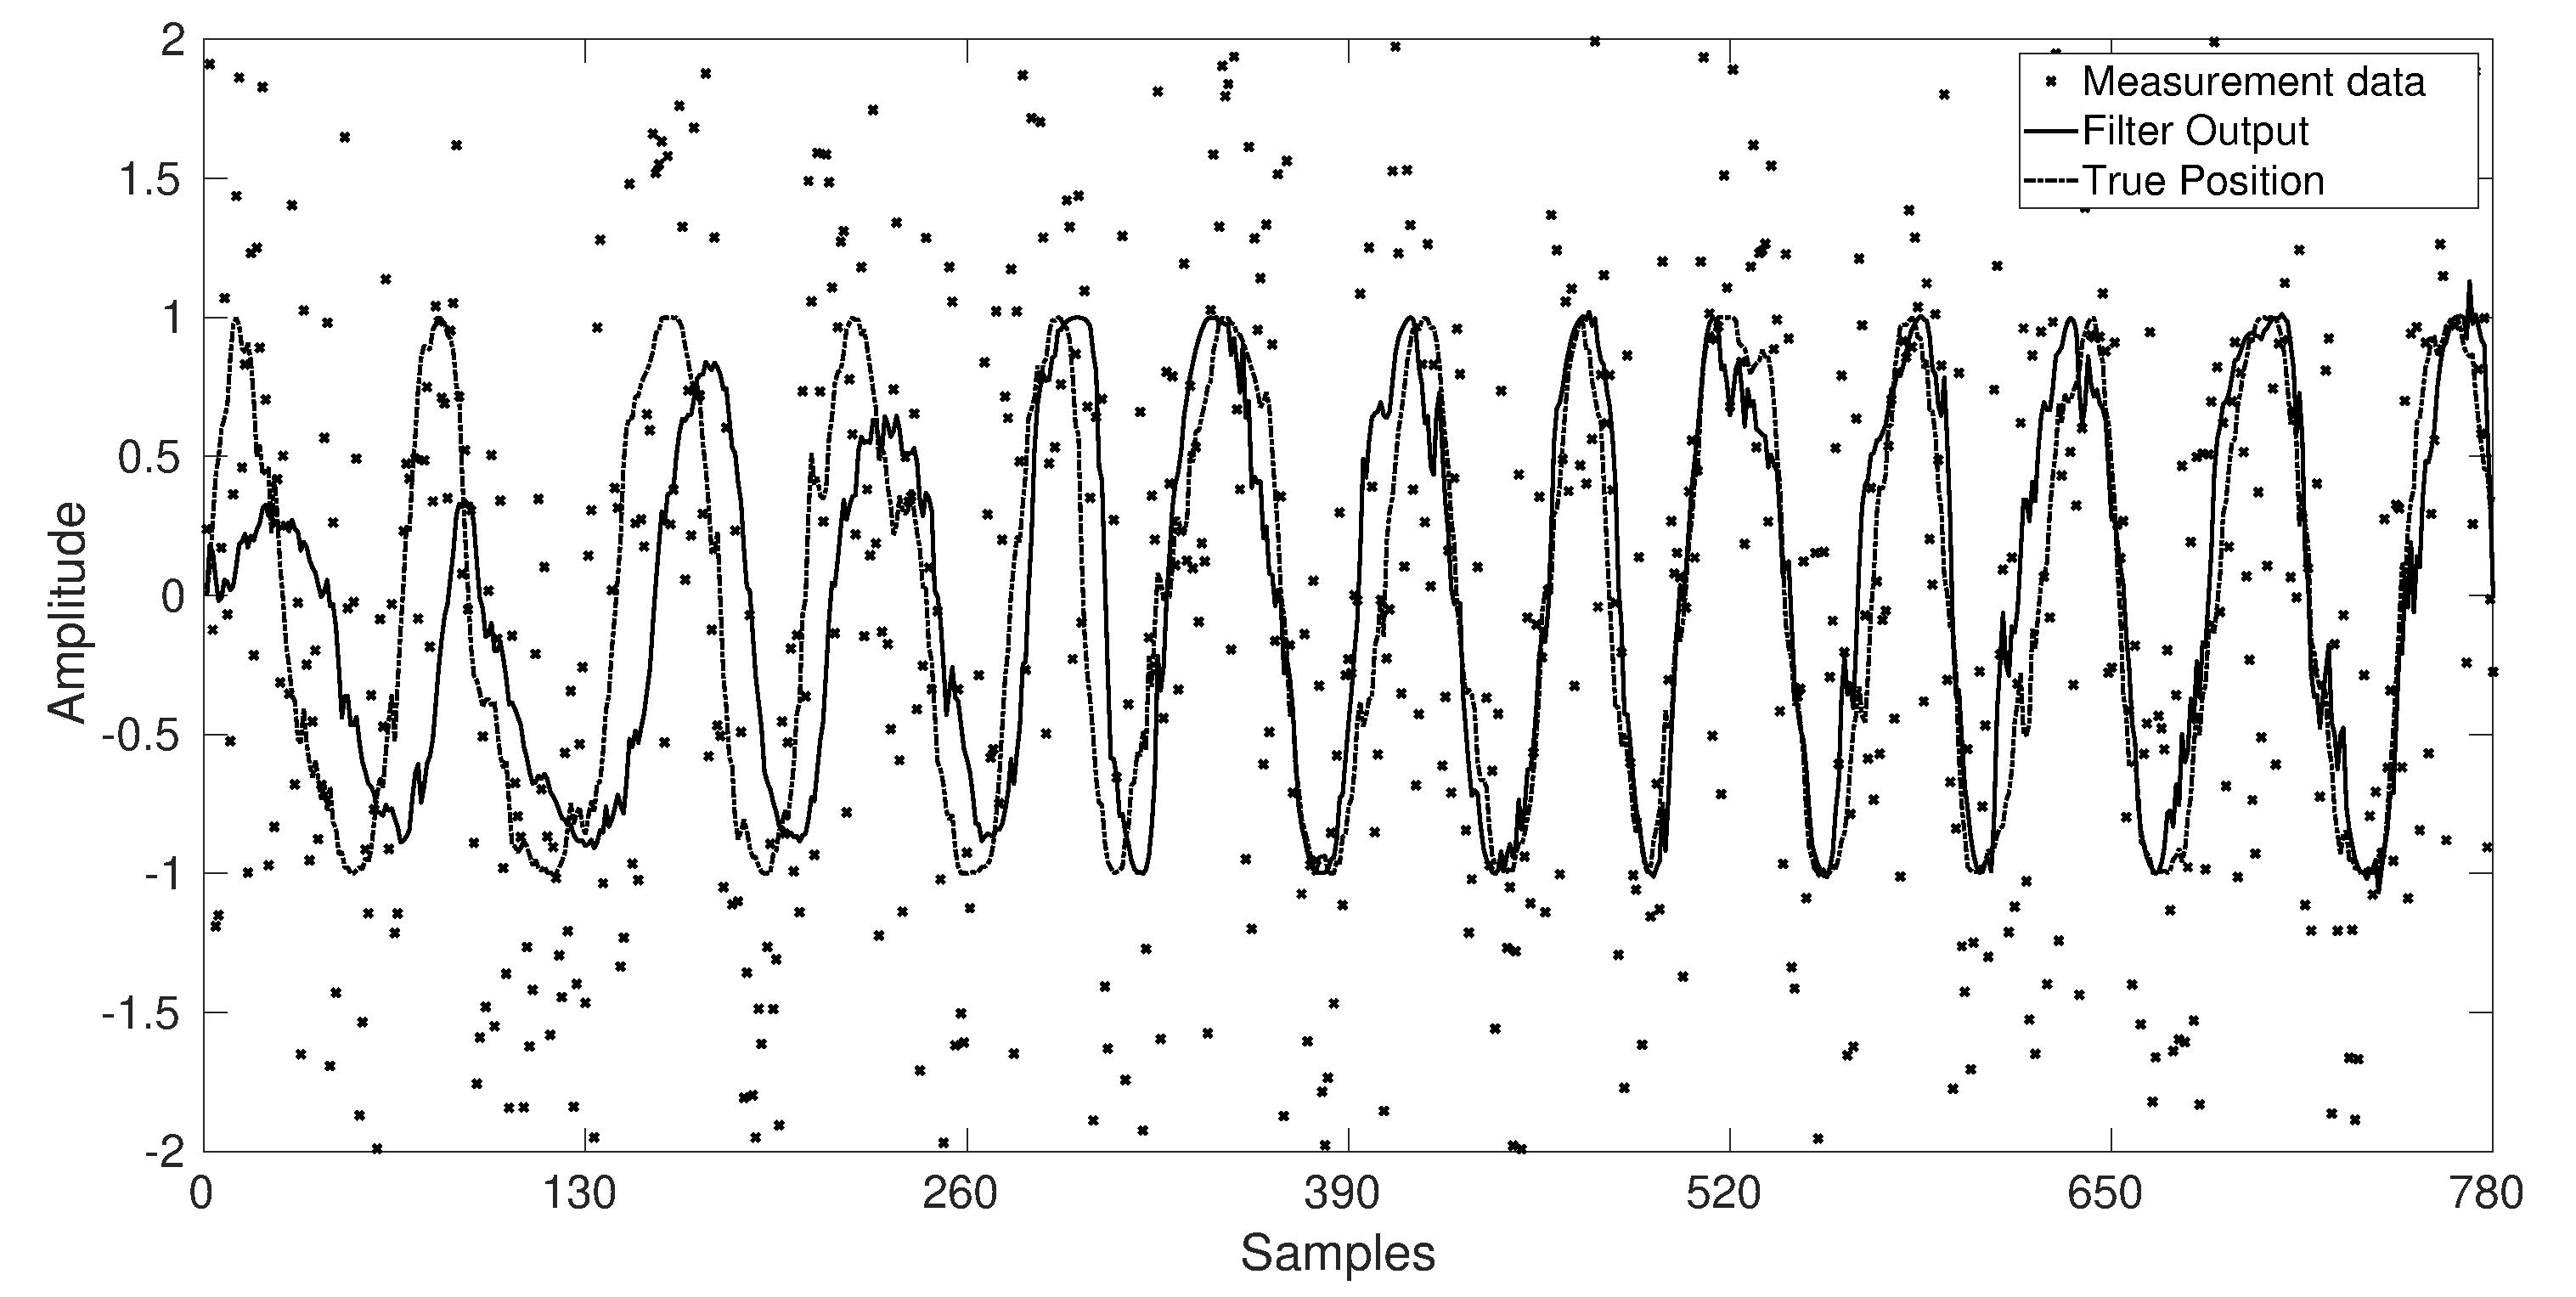
\includegraphics[width = \textwidth]{./Figures/ratio2.eps}
	\caption{EKF prediction for R = 0.1 and Q = 0.001}
	\label{fig:EKF rat2}
\end{figure} 
\quad \\
%R = 0.03 Q = 0.001
\begin{figure}[hb!]
\centering
	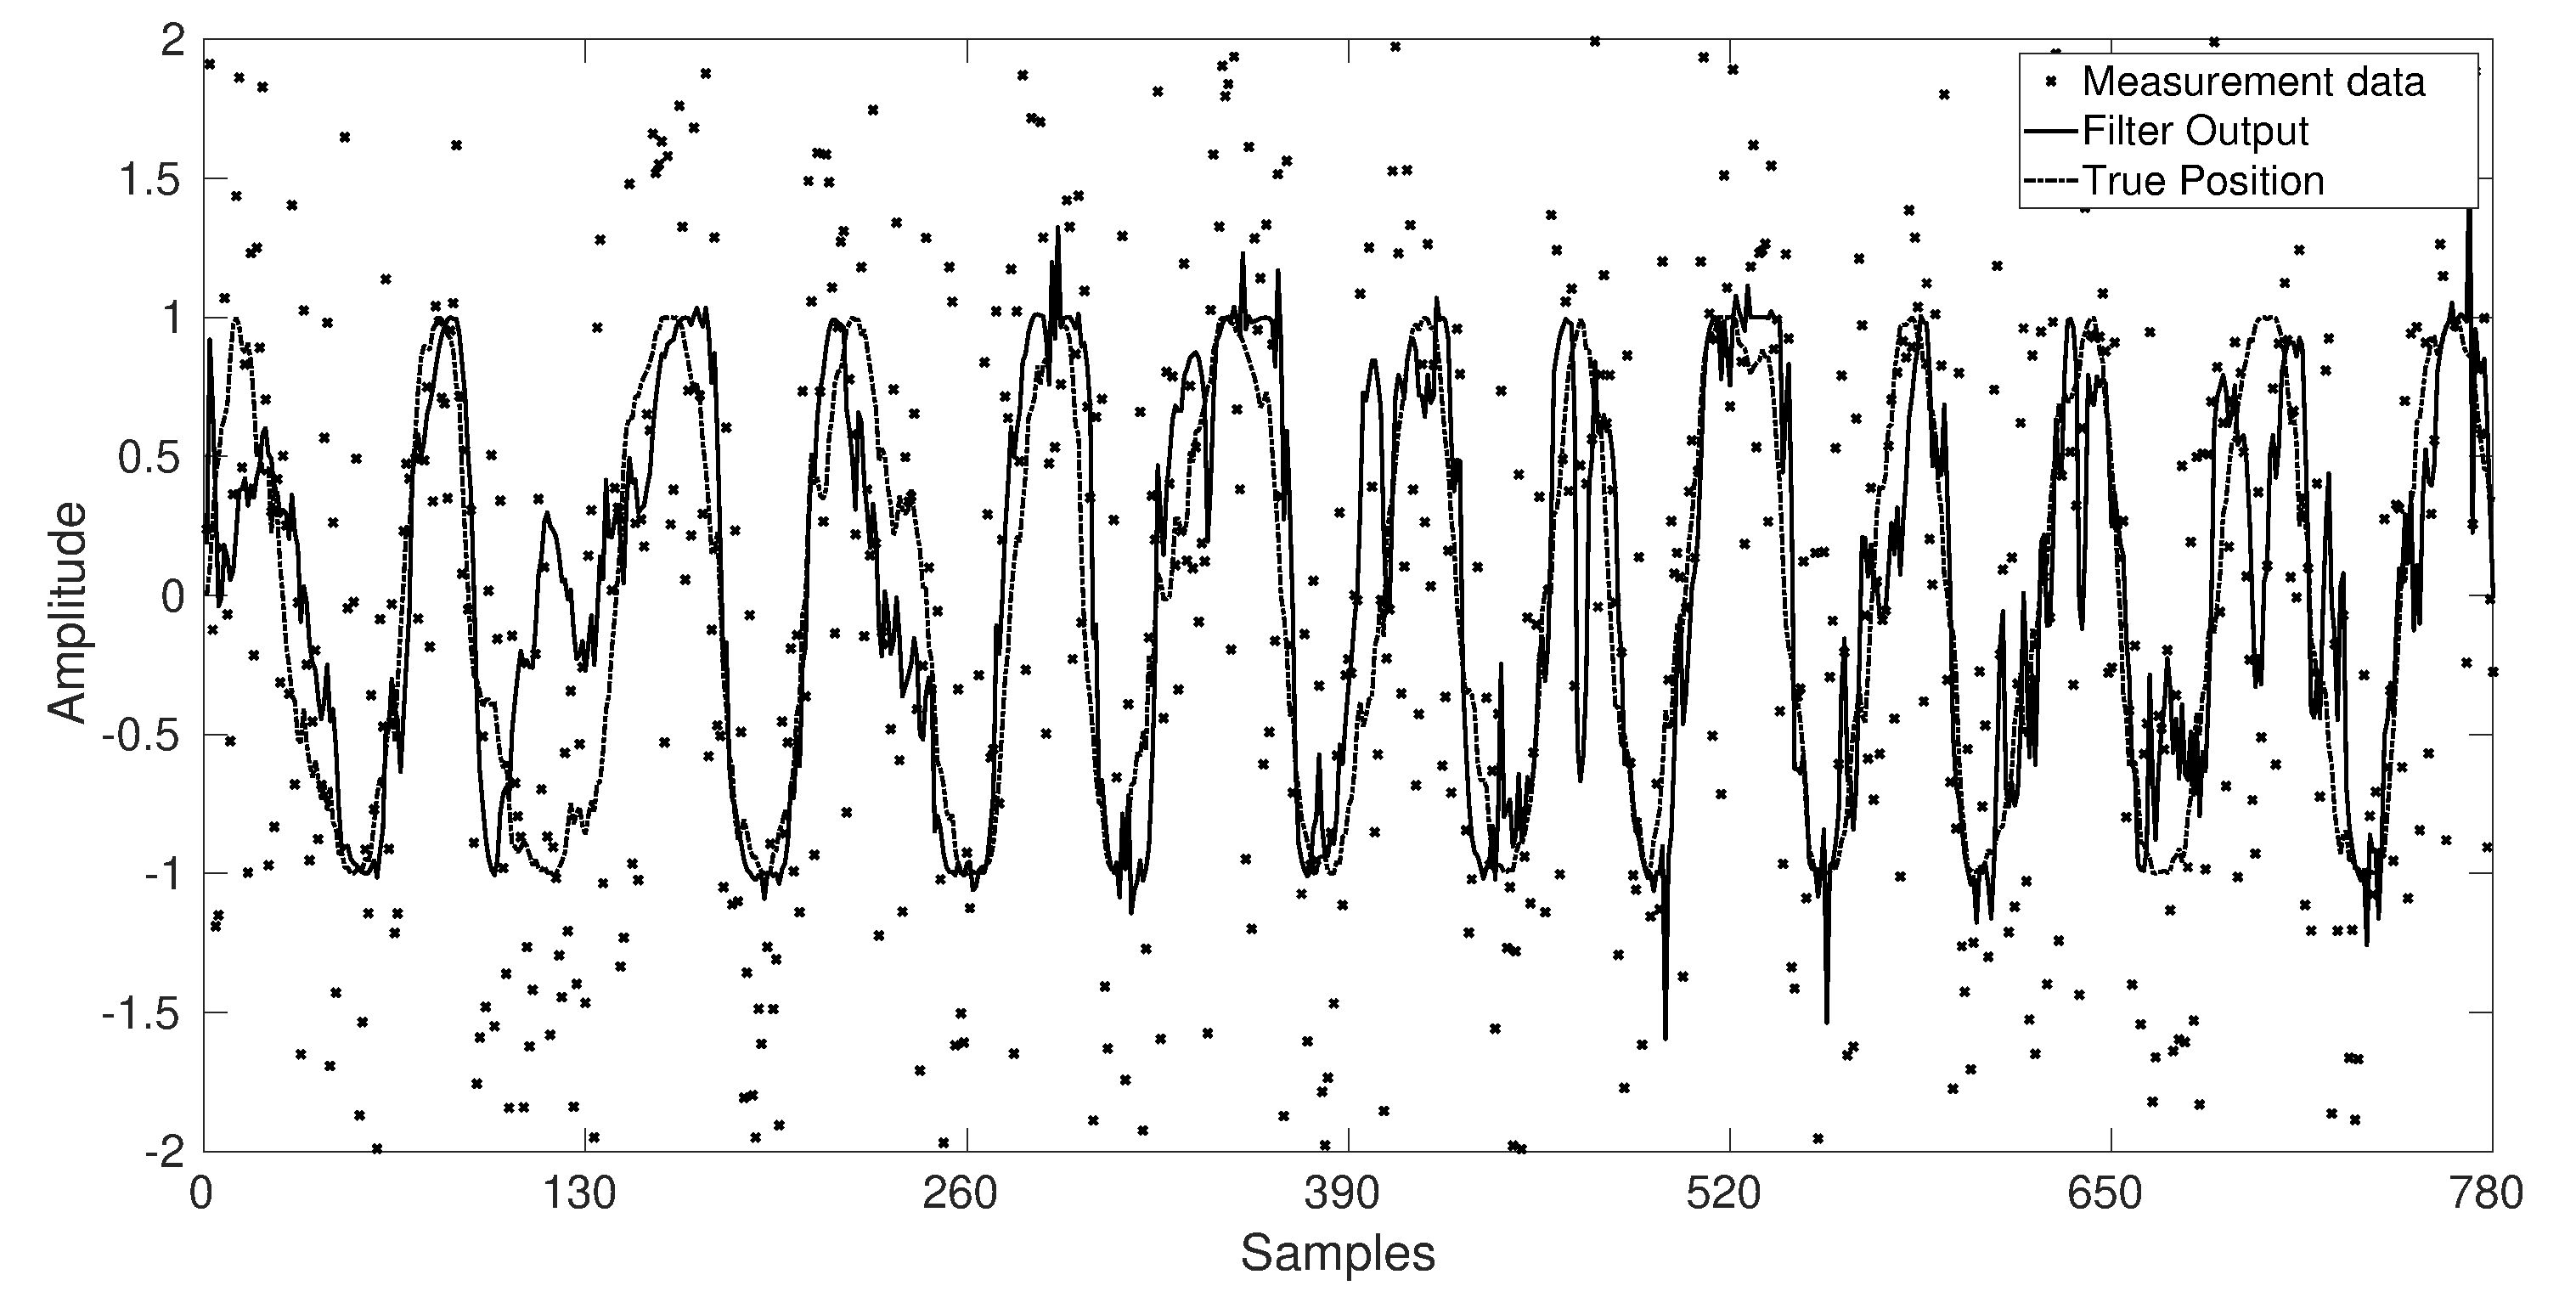
\includegraphics[width = \textwidth]{./Figures/ratio3.eps}
	\caption{EKF prediction for R = 0.03 and Q = 0.001}
	\label{fig:EKF rat3}
\end{figure} \newpage

\newpage
\section{Conclusion}
The goal of this lab was to implement EKF to track the position of a spool of thread unwinding in a machine. To track the position of the thread, a 1D sinusoidal model was designed and its model parameter equations were derived. The implementation was done on MATLAB. Sensor measurement readings were given in "sin-data.txt". \\
\\
To observe the effects of dynamic noise and measurement noise on the filter performance, the measurement noise, R was varied while keeping the dynamic noise, Q set at 0.001. With the decrease in R, EKF filter output inclined towards measurement reading and further away from true position.\textbf{ An acceptable performance was achieved for the ratio R = 0.1 and Q = 0.001}. \\
\\
Thus the EKF can be applied to a non-linear function like the sinusoidal signal by linearizing the equations using Taylor series.
\section*{References}
[1] \url{http://cecas.clemson.edu/~ahoover/ece854/lecture-notes/lecture-ekf-sine.pdf} \\
\quad \\
\noindent 
[2] \url{http://cecas.clemson.edu/~ahoover/ece854/lecture-notes/lecture-ekf.pdf} \\
\quad \\
\noindent
[3] \url{https://towardsdatascience.com/extended-kalman-filter-43e52b16757d}

\newpage
\section*{Appendix}

\subsection*{MATLAB Code}
%1D sinusoidal EKF
\lstinputlisting{../asg5.m}
%--------------------------------------------------------------------------------------------------------

\end{document}
